\documentclass[11pt]{article}

\usepackage[letterpaper,margin=0.82in,top=0.78in,bottom=0.82in]{geometry}
\usepackage[T1]{fontenc}
\usepackage{lmodern}
\usepackage{microtype}
\usepackage{graphicx}
\usepackage{booktabs}
\usepackage{enumitem}
\usepackage{caption}
\usepackage{subcaption}
\usepackage{titlesec}
\usepackage{fancyhdr}
\usepackage{xcolor}
\usepackage{hyperref}
\usepackage{parskip}
\usepackage{ragged2e}
\usepackage{float}
\usepackage{array}

\definecolor{skkublue}{HTML}{000000}
\definecolor{skkugreen}{HTML}{8DC63F}
\definecolor{textgray}{HTML}{000000}
\definecolor{rulegray}{HTML}{D9DDE3}

\hypersetup{
  colorlinks=true,
  linkcolor=black,
  urlcolor=black,
  citecolor=black,
  pdfauthor={Jeonghyun Park},
  pdftitle={Pneumatic Morphing Wheel: Design Exploration}
}

\setlength{\parindent}{0pt}
\setlength{\parskip}{0.52em}
\setlist[itemize]{leftmargin=1.4em,itemsep=0.2em,topsep=0.35em}

\titleformat{\section}
  {\Large\bfseries\color{skkublue}}
  {\thesection.}{0.45em}{}
  [\vspace{0.12em}\color{rulegray}\titlerule]
\titleformat{\subsection}
  {\large\bfseries\color{textgray}}
  {\thesubsection}{0.45em}{}

\captionsetup{font=small,labelfont=bf,labelsep=period,justification=centering}
\captionsetup[subfigure]{font=small,labelfont=bf}

\setlength{\headheight}{22pt}
\pagestyle{fancy}
\fancyhf{}
\fancyhead[L]{\small\color{textgray}Pneumatic Morphing Wheel}
\fancyhead[R]{\small\color{textgray}Design Exploration}
\fancyfoot[C]{\small\thepage}
\renewcommand{\headrulewidth}{0.35pt}
\renewcommand{\headrule}{\hbox to\headwidth{\color{rulegray}\leaders\hrule height \headrulewidth\hfill}}

\newcommand{\statebox}[2]{%
  \begin{minipage}[t]{0.47\textwidth}
    \vspace{0pt}
    {\bfseries\color{skkublue}#1}\\[-0.1em]
    #2
  \end{minipage}
}

\begin{document}

% -----------------------------------------------------------------------------
% Cover
% -----------------------------------------------------------------------------
\hypersetup{pageanchor=false}
\begin{titlepage}
\thispagestyle{empty}

% Put the exact official/user-provided logo in figures/skku_logo.png.
% The report intentionally falls back to plain text rather than using an
% approximated or recreated university mark.
\IfFileExists{figures/skku_logo.png}{%
  
\includegraphics[width=0.48\textwidth]{figures/skku_logo.png}
}{%
  {\sffamily\bfseries\large\color{skkublue}SUNGKYUNKWAN UNIVERSITY}
}

\vspace{1.2cm}
{\color{skkublue}\rule{\textwidth}{1.4pt}}

\vspace{1.0cm}
{\fontsize{28}{32}\selectfont\bfseries Pneumatic Morphing Wheel}\par
\vspace{0.3cm}
{\fontsize{20}{24}\selectfont\color{textgray}Design Exploration}\par

\vspace{1.5cm}
\begin{minipage}{0.82\textwidth}
\large
\textbf{Author}\\
Jeonghyun Park

\vspace{0.75cm}
\textbf{Project}\\
Morphing Wheel Using Pneumatic \& Locking Structure

\vspace{0.75cm}
\textbf{Institution}\\
Soft Robotics Laboratory\\
Sungkyunkwan University
\end{minipage}

\vfill
{\color{rulegray}\rule{\textwidth}{0.8pt}}\\[0.35cm]
{\small\color{textgray}Technical design report}
\end{titlepage}
\hypersetup{pageanchor=true}

\pagenumbering{arabic}
\setcounter{page}{1}

% -----------------------------------------------------------------------------
\section*{Abstract}
\addcontentsline{toc}{section}{Abstract}
This report explores the design of a pneumatic morphing wheel capable of transitioning between multiple mechanical states to improve mobility across variable terrain. The concept combines a soft inner pneumatic structure with an outer mechanical system that can compress and stiffen when air is removed. When airflow is allowed, the wheel becomes compliant and adaptable to obstacles; when air is extracted, the structure compresses and increases stiffness, enabling more stable rolling.

The report first examines the current prototype design, identifying key limitations including manufacturing complexity, unpredictable deformation, and integration challenges with torque transmission. A redesigned concept is then proposed that introduces guided deformation grooves, spring-assisted structural support, and deformation limiters to improve structural stability and repeatability.

System-level integration is also considered. Rather than transmitting torque through the pneumatic hub, a chain-driven system---similar to a bicycle drivetrain---is proposed. This configuration allows torque to be applied externally while a rotary pneumatic joint delivers airflow through the wheel hub without interference.

Finally, the design is compared with NASA's airless superelastic wheel technology, highlighting alternative strategies for achieving terrain adaptability without pneumatic pressure. Potential applications in robotic exploration and off-road mobility are discussed along with recommended experiments for evaluating the redesigned concept.

\section{Motivation and Design Concept}
Conventional wheels are typically designed with fixed geometry and stiffness. While rigid wheels are efficient on smooth surfaces, they often struggle on rough terrain. In such conditions, rigid wheels may lose traction, experience high shock loads, or fail to conform to obstacles.

The goal of this project is to explore a morphing wheel capable of adapting its mechanical properties depending on terrain conditions. The wheel is designed to transition between two primary operating states:

\vspace{0.25em}
\statebox{Compliant State (Unlocked)}{The wheel structure is flexible and deformable, allowing it to adapt to uneven terrain. Increased deformation can create a larger contact patch and improve traction.}
\hfill
\statebox{Stiff State (Locked)}{The structure compresses and becomes more rigid, maintaining a more stable geometry and reducing unwanted deformation during rolling.}
\vspace{0.45em}

This multi-state capability is intended to combine two typically conflicting properties:
\begin{itemize}
  \item efficient rolling on smooth terrain;
  \item improved traction and obstacle negotiation on rough terrain.
\end{itemize}

\subsection*{Why Pneumatics?}
Pneumatics were initially selected as the actuation mechanism because air pressure provides a relatively simple method for controlling compliance. By adjusting internal pressure, deformation can be distributed across the wheel volume rather than concentrated at a single mechanical joint. This can produce smoother transitions between states and supports rapid prototyping using relatively simple tubing, valves, and chambers.

\section{Current Design}
\subsection{Architecture}
The current prototype consists of a soft inner structure surrounded by a deformable outer wheel shell.

\begin{figure}[H]
  \centering
  \begin{subfigure}[b]{0.46\textwidth}
    \centering
    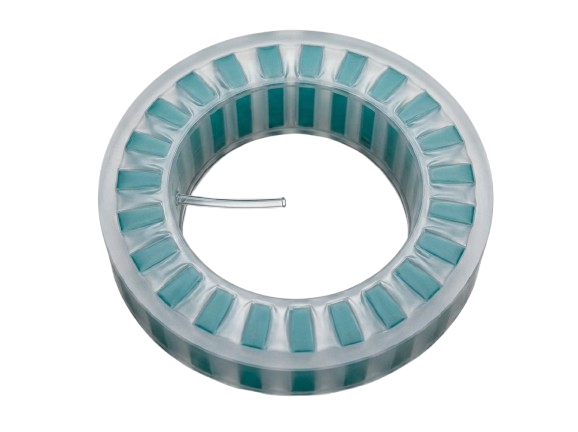
\includegraphics[width=\linewidth]{figures/prototype_unassembled.png}
  \end{subfigure}\hfill
  \begin{subfigure}[b]{0.46\textwidth}
    \centering
    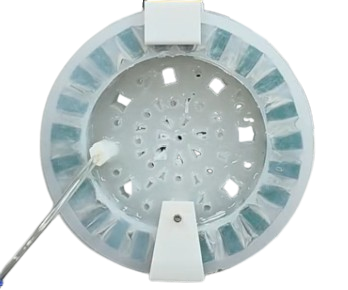
\includegraphics[width=\linewidth]{figures/prototype_assembled.png}
  \end{subfigure}
  \caption{Morphing wheel prototype. Photographs by author.}
  \label{fig:prototype}
\end{figure}

A ring of pneumatic chambers is distributed around the wheel circumference. These chambers can be pressurized or vented to influence the structural behavior of the wheel.

The wheel transitions between different mechanical states through airflow control. When airflow pathways are open, air can move between chambers, allowing the pneumatic structure to deform more freely. In this condition, the wheel becomes more compliant and better able to adapt to irregular terrain.

When air is removed or airflow is restricted, the pneumatic chambers collapse inward. This inward collapse increases the structural rigidity of the wheel and creates a stiffer configuration that resists further deformation.

This ability to transition between compliant and stiff configurations demonstrates how geometrically designed structures can produce multiple mechanical states, a principle often explored in transformable and origami-inspired mechanical systems.

\subsection{Strengths of the Current Design}
The current prototype demonstrates several important advantages:
\begin{itemize}
  \item \textbf{Multi-state mechanical behavior.} The wheel can transition between compliant and stiff configurations.
  \item \textbf{Conceptual simplicity.} The stiffness transition is controlled using air pressure rather than a large number of independent mechanical linkages.
  \item \textbf{Rapid iteration.} A tubing-, valve-, and chamber-based architecture is comparatively straightforward to assemble and modify while testing changes in geometry.
\end{itemize}

For comparison, multi-cable morphing-wheel concepts can provide highly controlled shape change but introduce additional routing, tensioning, and integration requirements.

\begin{figure}[H]
  \centering
  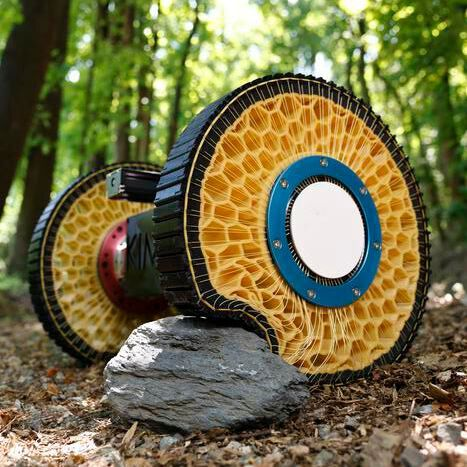
\includegraphics[width=0.52\textwidth]{figures/multicable_morphing_wheel.png}
  \caption{Multi-cable morphing wheel. Image from ``Groundbreaking Morphing Wheel Technology for Enhanced Mobility,'' by Sung-Hyuk Park and Dong Il Park, \textit{Lab-Worldwide}, 3 Sept. 2024.}
  \label{fig:multicable}
\end{figure}

\section{Limitations of the Current Design}
Although the prototype demonstrates the feasibility of the concept, several limitations were identified during development.

\subsection{Complex and Time-Consuming Assembly}
The fabrication process of the current prototype is highly time-consuming. Each pneumatic chamber must be individually attached to a plastic film using adhesive. This process is necessary to maintain consistent spacing between the structural elements, but it significantly increases assembly time and reduces manufacturing efficiency.

Because the chambers must be manually positioned and attached, the process also introduces variability in spacing and alignment. This makes the overall structure difficult to reproduce consistently.

\subsection{Difficulty Integrating a Motor or Drive Mechanism}
The soft inner pneumatic structure improves morphability, but it also creates challenges when integrating a motor or drive shaft. Since the central region of the wheel is highly compliant, it becomes difficult to securely attach a motor or transmit torque through the wheel hub.

A stable and rigid mounting interface is typically required for motor integration, but the softness of the inner structure complicates this requirement.

\subsection{Instability Due to Excessive Compliance}
Because the inner structure is extremely soft, the wheel can bend along unintended axes when subjected to external loads. Under significant loading, this may lead to structural instability.

One possible response would be to increase structural thickness or wheel diameter to improve load distribution. However, both approaches introduce new design challenges, including increased size, weight, and mechanical complexity.

\subsection{Over-Reliance on Soft Polymer Materials}
The current design relies heavily on soft polymer materials to achieve deformability. While this allows the wheel to morph easily, it also introduces uncertainty in how the structure behaves during deformation.

When air is removed from the pneumatic chambers, the wheel shrinks and folds inward. Because the structure is primarily governed by soft materials, the folding pattern can become unpredictable. This unpredictability makes it difficult to ensure controlled deformation and consistent performance.

\begin{figure}[H]
  \centering
  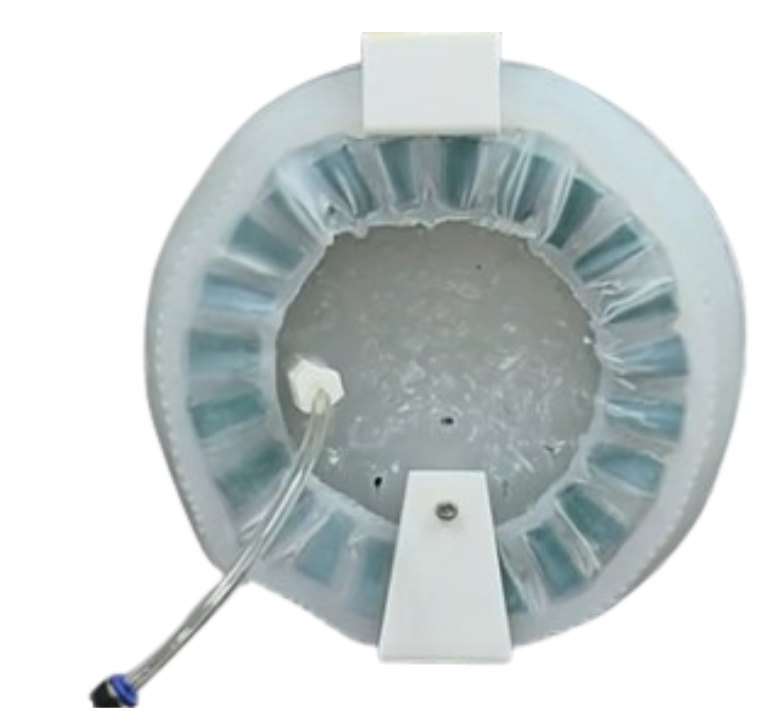
\includegraphics[width=0.56\textwidth]{figures/wrinkling_80kPa.png}
  \caption{Non-uniform wrinkling deformation of the membrane under 80 kPa vacuum pressure. Photograph by author.}
  \label{fig:wrinkling}
\end{figure}

\section{Proposed Design Improvements}
To address the limitations identified in the current prototype, several design improvements are proposed.

\subsection{Guided Deformation Using Grooves}
The redesigned wheel introduces grooves or pre-defined compliant regions along the outer wheel structure to guide how the wheel compresses when air is removed.

\begin{figure}[H]
  \centering
  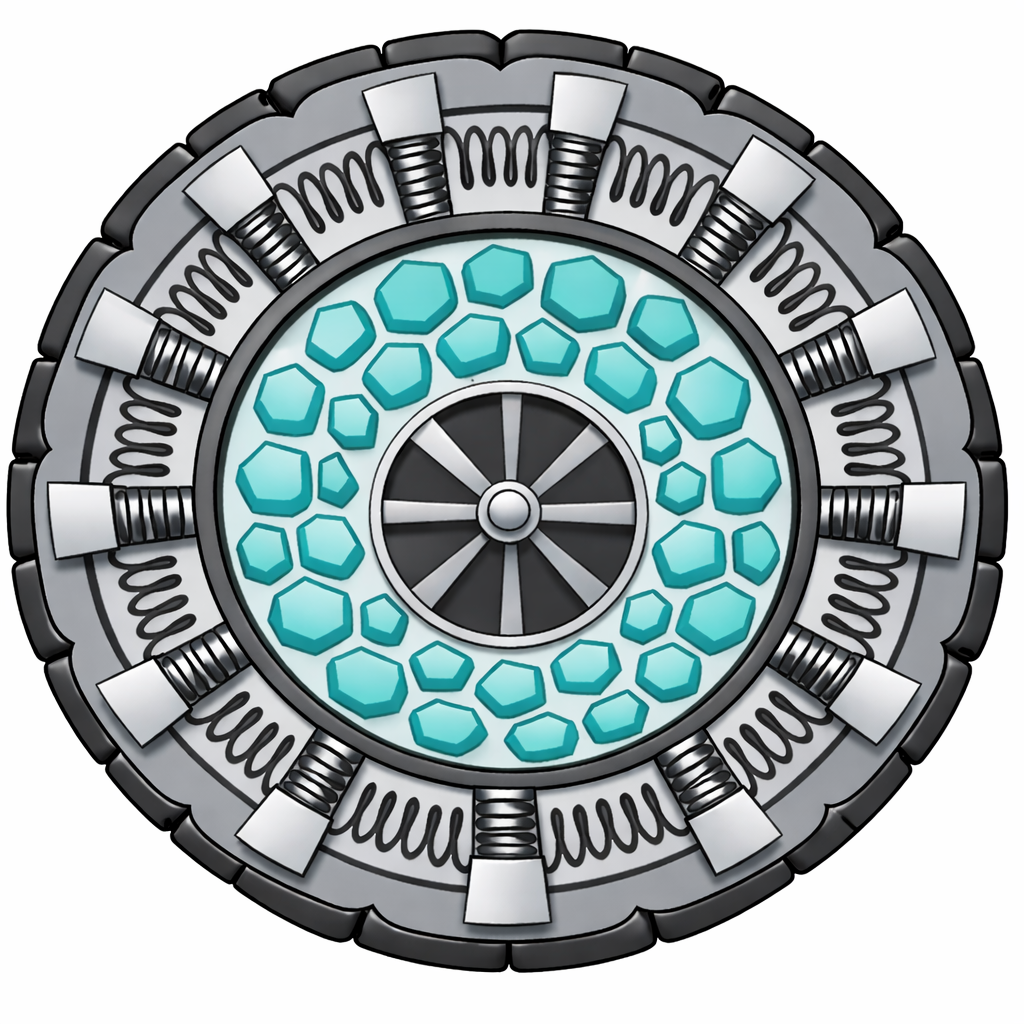
\includegraphics[width=0.58\textwidth]{figures/creased_spring_concept.png}
  \caption{Conceptual rendering of a pre-creased outer wheel geometry intended to promote more uniform and predictable radial collapse. AI-generated image by author.}
  \label{fig:creased}
\end{figure}

Instead of collapsing randomly, the wheel is intended to fold along predefined deformation paths. Guided deformation could provide several advantages:
\begin{itemize}
  \item controlled folding behavior;
  \item reduced risk of irregular wrinkling;
  \item more consistent wheel geometry during compression;
  \item reduced likelihood of debris becoming trapped in deep, uncontrolled folds.
\end{itemize}

\subsection{Spring-Assisted Structural Support and Recoverability}
A key improvement in the proposed redesign is the integration of spring elements within the wheel structure. The goal is to combine structural support with controlled deformability while improving shape recovery after compression.

Springs provide several potential mechanical advantages for this application:
\begin{itemize}
  \item \textbf{Recoverable deformation.} Elastic energy stored in the springs can help the wheel return toward its original geometry after deformation.
  \item \textbf{Distributed load support.} A circumferential spring network can spread loads across multiple structural elements, reducing localized stress concentrations.
  \item \textbf{Improved durability.} Sharing load among multiple structural elements may reduce repeated local deformation of the soft polymer components.
  \item \textbf{Improved lateral stability.} A distributed spring network can provide resistance against bending along unintended axes of the wheel.
\end{itemize}

In addition to improving structural behavior, the spring network could simplify manufacturing. The current prototype relies on plastic film and adhesive assembly to maintain spacing between structural components. By contrast, a spring-based structure can help maintain spacing mechanically, reducing dependence on manually positioned film attachments.

Another potential advantage is that the locking behavior could become less dependent on high-friction surface contact. Mechanical preload or geometric constraint within the spring network could supplement the pneumatic locking mechanism and improve repeatability.

\subsection{Limiting Diameter Reduction During Suction}
When air is removed from the pneumatic chambers, the wheel compresses and transitions into a stiffer configuration. However, excessive shrinkage could reduce ground clearance and negatively affect vehicle dynamics.

The redesigned structure therefore incorporates constraints that allow the wheel to stiffen while limiting excessive diameter reduction. This helps preserve a usable wheel geometry during the locking transition.

\subsection{Limiting Maximum Deformation}
Structural limiters can also be incorporated to prevent excessive compression and excessive deformation of the soft material. These features can provide more reliable hard points for attaching motor, axle, or metallic components.

By defining a minimum allowable geometry, the limiters can help the wheel stiffen under suction without collapsing into an unstable configuration.

\section{System Integration: Torque Transmission and Air Delivery}
A major engineering challenge is integrating both torque transmission and pneumatic airflow in a rotating wheel.

Instead of transmitting torque through the pneumatic hub, the proposed system uses a chain-driven drivetrain similar to a bicycle mechanism. In this configuration:
\begin{itemize}
  \item torque is applied through an external chain drive;
  \item the central hub is reserved for pneumatic airflow;
  \item a rotary pneumatic joint supplies air to the rotating wheel.
\end{itemize}

\begin{figure}[H]
  \centering
  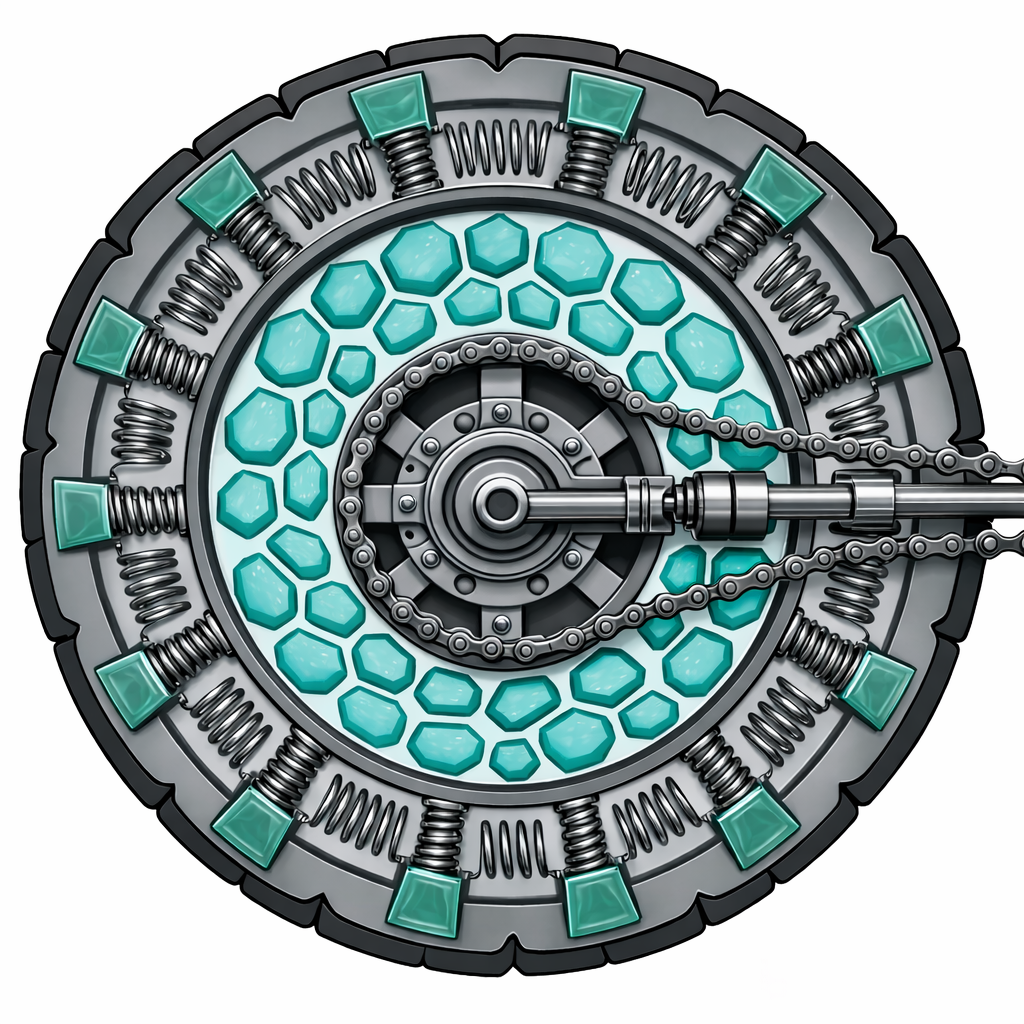
\includegraphics[width=0.69\textwidth]{figures/drivetrain_pneumatic_concept.png}
  \caption{Conceptual rendering of drivetrain--pneumatic integration. Torque is transmitted through an external chain drive while a rotary pneumatic joint supplies airflow through the central hub. AI-generated image by author.}
  \label{fig:drivetrain}
\end{figure}

This architecture separates the two functions that otherwise compete for space at the hub. The rotary joint allows air to flow from a stationary pneumatic source to the rotating wheel while preserving continuous rotation.

\section{Inspiration from Existing Research}
The morphing-wheel concept explored in this project shares similarities with deformable wheel technologies developed for planetary exploration. In particular, NASA has investigated airless and superelastic rover wheel designs that provide pneumatic-like compliance without relying on internal air pressure.

One example is NASA's Superelastic Tire, which uses a woven metallic mesh structure. This design allows the wheel to deform when encountering obstacles while maintaining structural integrity. Because the structure does not rely on internal pneumatic pressure, it is inherently resistant to puncture-related failure.

\begin{figure}[H]
  \centering
  \begin{subfigure}[b]{0.49\textwidth}
    \centering
    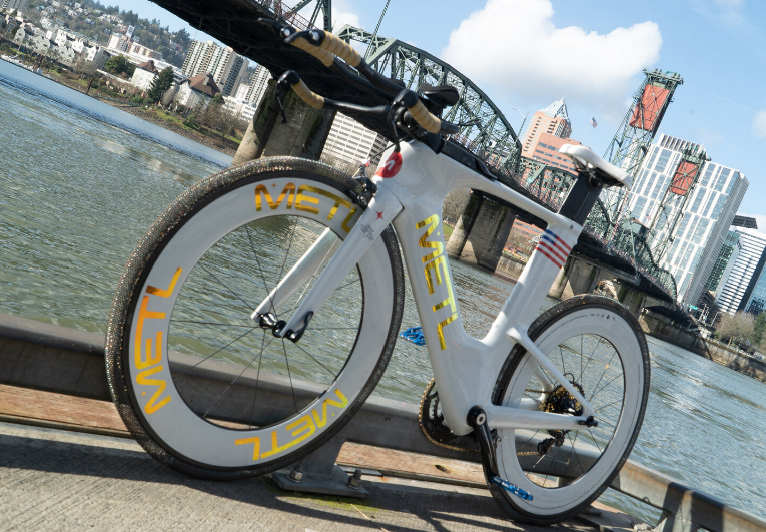
\includegraphics[width=\linewidth]{figures/nasa_bicycle.png}
  \end{subfigure}\hfill
  \begin{subfigure}[b]{0.49\textwidth}
    \centering
    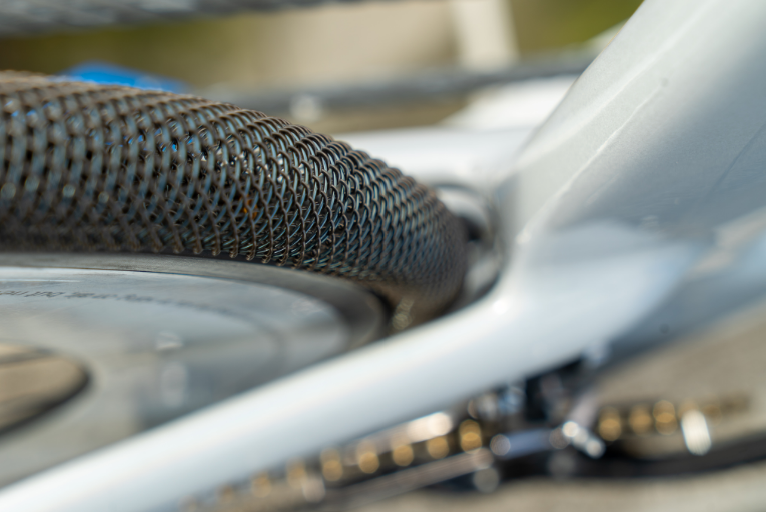
\includegraphics[width=\linewidth]{figures/nasa_mesh.png}
  \end{subfigure}
  \caption{NASA airless tire technology: bicycle implementation (left) and close-up of the alloy mesh structure (right). Images from NASA's Airless Tire Technology, NASA Technology Transfer Program.}
  \label{fig:nasa}
\end{figure}

These designs highlight an important principle for mobility systems operating in harsh environments: structural compliance and durability can be achieved through the architecture and material system of the wheel itself.

While NASA's approach focuses on material-based compliance through metallic mesh structures, the morphing wheel in this project explores pneumatic control as a method for switching between mechanical states. Pneumatic actuation provides an additional control input that can change structural behavior during operation.

The NASA design also suggests an alternative direction for future development. Rather than relying solely on vacuum-driven locking, the spring network could potentially be mechanically preloaded or constrained to change the wheel's effective structural resistance. Such an approach could reduce dependence on pneumatic hardware in applications where pumps, hoses, or pressure maintenance are undesirable.

\section{Potential Applications}
The morphing-wheel concept may be useful in environments where terrain conditions vary significantly. Potential applications include:
\begin{itemize}
  \item robotic exploration vehicles;
  \item off-road mobility systems;
  \item vehicles operating in sand, mud, or loose terrain.
\end{itemize}

For example, when a vehicle becomes stuck in sand or attempts to climb a steep slope, switching the wheel to a more compliant state could increase ground contact and improve traction.

Wheelchair applications were also considered. However, the additional pneumatic components may increase system weight and complexity. Because wheelchair performance is sensitive to weight distribution, package size, reliability, and user effort, robotic exploration platforms may represent a more practical near-term application for the current architecture.

\section{Proposed Experimental Evaluation}
To evaluate the redesigned wheel concept more rigorously, several experiments are proposed.

\subsection*{Obstacle Step Test}
This test would measure the wheel's ability to overcome obstacles of varying heights. By gradually increasing step height, the experiment could compare how compliant and stiff states affect obstacle-climbing performance and terrain adaptability.

\subsection*{Compression Test}
Compression testing would measure the relationship between applied load and wheel deformation. A force--displacement measurement would also help identify the point at which structural limiters engage and begin providing additional support.

\subsection*{Fatigue Test}
Repeated cycles of locking and unlocking would evaluate long-term durability, including potential material fatigue, seal degradation, spring degradation, and structural damage.

\subsection*{Rolling Resistance Test}
Rolling resistance could be measured to compare energy efficiency between stiff and compliant configurations and determine whether the locked state improves rolling efficiency on flat surfaces.

\subsection*{Lateral Stability Test}
This experiment would evaluate the wheel's resistance to bending along unintended axes. Applying controlled lateral loads would help determine whether the redesigned spring-supported architecture improves stability.

\section{Conclusion}
This project explored the design of a pneumatic morphing wheel capable of adapting its mechanical properties to different terrain conditions. By combining a soft pneumatic structure with a controllable locking mechanism, the wheel is intended to transition between a compliant state for obstacle negotiation and a stiffer state for more stable rolling. This multi-state behavior aims to balance terrain adaptability with rolling performance, two objectives that are difficult to achieve simultaneously with a conventional fixed-stiffness wheel.

Evaluation of the current prototype revealed several important limitations, including complex manufacturing processes, difficulty integrating torque transmission, structural instability under load, and unpredictable deformation due to heavy reliance on soft polymer materials. These limitations motivated a redesigned concept.

The proposed redesign introduces guided deformation features, spring-assisted structural support, and mechanisms that limit excessive compression while maintaining recoverability. The proposed drivetrain configuration---using chain-based torque transmission with a rotary pneumatic joint at the hub---also provides a practical way to separate torque delivery from airflow routing.

Inspired by existing airless and superelastic wheel research, the project additionally considers whether mechanical preload of the spring network could supplement or eventually replace pneumatic stiffness control. Overall, the design exploration suggests that controlled structural deformation is a promising direction for adaptive mobility systems. Future work should refine the mechanical architecture and evaluate the concept through controlled force--displacement, durability, rolling, and terrain tests.

\clearpage
\section*{Works Cited}
\addcontentsline{toc}{section}{Works Cited}
\small
\begin{enumerate}[label={[\arabic*]},leftmargin=2.2em]
  \item Park, Sung-Hyuk, and Dong Il Park. ``Groundbreaking Morphing Wheel Technology for Enhanced Mobility.'' \textit{Lab-Worldwide}, 3 Sept. 2024.
  \item NASA Technology Transfer Program. ``NASA's Airless Tire Technology.'' Accessed 10 Mar. 2026.
  \item Howell, Larry L., Spencer P. Magleby, and Brian M. Olsen. \textit{Handbook of Compliant Mechanisms}. Wiley, 2013.
  \item Lee, H., et al. ``Superelastic Tire for Mars Exploration.'' NASA Glenn Research Center, 2017.
  \item McGee, Kate. ``NASA's Superelastic Tire Is Made from Shape Memory Alloy.'' \textit{Engadget}, 2017.
  \item Pellegrino, Sergio. ``Deployable Structures.'' In \textit{Springer Handbook of Structural Engineering}. Springer, 2014.
  \item Tolley, Michael T., et al. ``Origami-Inspired Self-Folding Structures.'' \textit{Science Robotics}, vol. 2, 2017.
\end{enumerate}

\end{document}
